%ju 28-Mai-22 FM_U04_Spannungsabfall_Mathebuch_Loesung.tex
\section{Spannungsabfall Übung 4
Mathebuch}\label{spannungsabfall-uebung-4-mathebuch}

Vgl. Mathebuch (\textcite{elbl:2016:technMa} S. 107)

\textbf{Aufgabe 1}

Schaltung Spannungsverlust

\begin{figure}[!ht]% hier: !ht
\centering
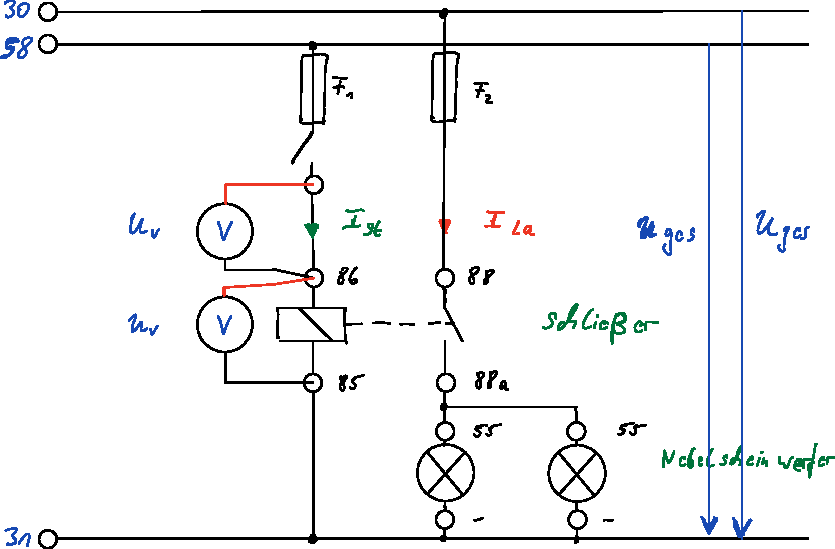
\includegraphics[width=0.65\textwidth]{images/Skizze/13_Spannungsverlust_Skizze.pdf}
\caption{Schaltung Spannungsverlust Aufgabe 1}
%\label{fig:}%% anpassen
\end{figure}

Nennquerschnitt Tabellenbuch (\textcite{bell:2021:tabellenbuchKfz} S. 280)

Spannungsfall Tabellenbuch (\textcite{bell:2021:tabellenbuchKfz} S. 280)

geg:

$l_1 = 0,8~m, l_2 = 1,6~m, l_{2}' = 1,6~m$

$U_{v_{l_1}} = 0,1 V, U_{v_{l_2}} = 0,1 V, U_{v_{l_2}}' = 0,1 V$

$P_{La_{22/23}}= 12~V/55~W, P = 55~W, U = 12~V$

$\rho = 0,0178~\frac{\Omega \cdot mm^2}{m} \,\text{(Kupfer)}$

ges:
$I, A_{l_1}, A_{Nenn}, J_{l_1}, A_{l_2}, J_{A_{l_2}}, J_{A_{l_2}}'$

Formel:

$P = U \cdot I \to I = \frac{P}{U}$

$U_{v_{l_1}} = \frac{\rho \cdot l_1 \cdot I}{A_{l_1}} \to A_{l_1} = \frac{\rho \cdot l_1 \cdot 2 \cdot I}{U_{v_{l_1}}}$

$J_{A_{l_2}} = \frac{I}{A_{Nenn}}$

$U_{v_{l_2}} = U_{v_{l_2}}' \to U_{v_{l_2}} = \frac{\rho \cdot l_2 \cdot I}{A_{l_2}} \to A_{l_2} = \frac{\rho \cdot l_2 \cdot I}{U_{v_{l_2}}}$

$J_{A_{l_2}} = J_{A_{l_2}}' \to J_{A_{l_2}} = \frac{I}{A_{Nenn}}$

Lösung:

$I = 4,5833~A$

$A_{l_1} = 1,3053~mm^2 \to A_{Nenn} = 1,5~mm^2$

$J_{l_1} = 6,1111~\frac{A}{mm^2}$

$A_{l_2} = 1,3053~mm^2 \to A_{Nenn} = 1,5~mm^2$

$J_{A_{l_2}} = J_{A_{l_2}}' = 3,0556~\frac{A}{mm^2}$

\textbf{Aufgabe 2}

geg:

$I = 165~A$

$l_{ges} = 1,7 + 3,4~m$ (zwei Kabel)

$U_{v_{max}} = 0,5~V$

$U_{k_{Bat}} = 11,2~V$

$\rho = 0,0178~\frac{\Omega \cdot mm^2}{m} \,\text{(Kupfer)}$

ges: $A_{mind}, A_{Nenn}, U_{v_{mind}}, U_{K_{st}}$

Formel:

$U_v = \frac{\rho \cdot l \cdot I}{A} \to A_{mind} = \frac{\rho \cdot l_{ges} \cdot I}{U_{v_{max}}}$

$U_{v_{mind}} = \frac{\rho \cdot l_{ges} \cdot I}{A_{mind}} \quad \text{vs.} \quad U_{v_{Nenn}} = \frac{\rho \cdot l_{ges} \cdot I}{A_{Nenn}}$

$U_{K_{st}} = U_{k_{Bat}} - U_{v_{Nenn}}$

Lösung:

$A = 29,9574~mm^2 \to A_{Nenn} = 35~mm^2$ (Nennquerschnitt)

$U_{v_{mind}} = 0,5~V \quad \text{vs.} \quad U_{v_{Nenn}} = 0,428~V$

$U_{K_{st}} = 10,772~V$
